\documentclass[compress]{beamer}
% \documentclass[handout]{beamer}

%% STYLES
%
% http://deic.uab.es/~iblanes/beamer_gallery/index_by_theme.html
%

%% USER GUIDE
%
% http://texdoc.net/texmf-dist/doc/latex/beamer/doc/beameruserguide.pdf
%

\mode<presentation>
{
  \usetheme{default}      
  \usecolortheme{beaver} 
  \usefonttheme{structuresmallcapsserif}  
  \setbeamertemplate{navigation symbols}{}
  \setbeamertemplate{caption}[numbered]
} 

%-----------------------------------%

\usepackage[english]{babel}
\usepackage[utf8x]{inputenc}
\usepackage{tikz}
\usetikzlibrary{arrows,petri,topaths,shapes,positioning}
\usepackage{tkz-berge}
\usepackage{verbatim}
\usepackage{color}
\usepackage{xparse}    % http://ctan.org/pkg/xparse
\usepackage{etoolbox}  % http://ctan.org/pkg/etoolbox
\usepackage[first=8, last=25]{lcg}

%-----------------------------------%

%% A (robust) Strike-Through [text] Command
\newcommand<>{\xcancel}[1]{%
    \tikz[baseline=(tocancel.base)]{
        \node[inner sep=0pt,outer sep=0pt] (tocancel) {#1};
        \only#2{\draw[red,thick] (tocancel.south west) -- (tocancel.north east); \draw[red,thick] (tocancel.north west) -- (tocancel.south east);}
    }%
}%

%% Basic Highlight Command
\newcommand<>{\hilight}[1]{\only#2{\colorbox{blue!40}}{#1}}

%% Random Number Generator
\newcommand{\rn}{%
\rand\arabic{rand}
}%

%-----------------------------------%

%% Network Maker Command
%
% Syntax:
%        \net{number of vertices}
%            {vertex-set}
%            {adjacency matrix}
%
% Matrix Syntax:
%               {x,1,0,0},
%               {-,x,1,1},
%               {-,-,x,1},
%               {-,-,-,x}
% ..for example.
%
\newcommand*{\net}[3]{%
%
% the vertex-set
\def\vertices{#2}
%
% the number of vertices
\def\n{#1}
%
% the adjacency-matrix
\def\weights{%
#3
};
%
% the radius of the circle 
\def\r{6.5}
%
% the width
\pgfmathparse{1.0*(\n)*\r}\let\wid\pgfmathresult
%
% \m:=(\n)-1 
\pgfmathparse{(\n)-1}\let\m\pgfmathresult
%
%%%%%%%%%%%%%%%%%%%%%%%%%%%%%%
%                            %
% First we draw the vertices %
%                            %
%%%%%%%%%%%%%%%%%%%%%%%%%%%%%%
%% If the vertex-set IS NOT GIVEN do this...
\ifdefempty{\vertices}
{%
\foreach \c in {0,1,...,\m} {%
\pgfmathparse{1.0*\c/(\n)*360}\let\ang\pgfmathresult;
\pgfmathparse{ 0.5*\wid/(\n)*cos(\ang) }\let\xx\pgfmathresult;
\pgfmathparse{ 0.5*\wid/(\n)*sin(\ang) }\let\yy\pgfmathresult;
\node[vertex] (\c) at (\xx,\yy) {\c};
}%
}%
%% If the vertex-set IS GIVEN do this...
{%
\foreach \i [count=\c from 0] in \vertices {%
\pgfmathparse{1.0*\c/(\n)*360}\let\ang\pgfmathresult;
\pgfmathparse{ 0.5*\wid/(\n)*cos(\ang) }\let\xx\pgfmathresult;
\pgfmathparse{ 0.5*\wid/(\n)*sin(\ang) }\let\yy\pgfmathresult;
\node[vertex] (\c) at (\xx,\yy) {\i};
}%
}%
%
%%%%%%%%%%%%%%%%%%%%%%%%%%%%%%%%%%%%%%%%%%%%%%%%
%                                              %
% Connect vertices with edges and draw weights %
%                                              %
%%%%%%%%%%%%%%%%%%%%%%%%%%%%%%%%%%%%%%%%%%%%%%%%
%% If the weights ARE NOT GIVEN do this...
\ifdefempty{\weights}
{%
\foreach \i in {0,1,...,\m} {%
\foreach \j in {\i,...,\m} {%
\ifnum \i=\j
{ }
\else 
\path[edge] (\i) -- (\j);  
\fi
}%
}%
}%
%% If the weights ARE GIVEN do this...
{%
\foreach \i [count=\row from 0] in \weights
{%
  \foreach \j [count=\col from 0] in \i
  {%
  \ifnum \row>\col
  {%
  }%
  \else
  {%
    \ifnum \row=\col
    {%
    }%
    \else
    {%
      \ifnum \j=0
      {%
      }%
      \else
      {%
        \ifnum \j=1
        {%
          \path[edge] (\row) -- (\col);  
        }%
        \else
        {%
          \path[edge] (\row) -- node[weight] {\j} (\col);  
        }%
        \fi
      }%
      \fi
    }%
    \fi
  }%
  \fi
  }%
}%
}%
%
%
%
% Practice Safe TeX
%
\let\n\undefined
\let\m\undefined
\let\r\undefined
\let\wid\undefined
\let\ang\undefined
\let\vertices\undefined
\let\weights\undefined
%
}%


%-----------------------------------%

%%%%%%%%%%%%%%%%%%%%%%%%%%%%%%%%%%%
%                                 %
% Vertex, Edge, and Weight Styles %
%                                 %
%%%%%%%%%%%%%%%%%%%%%%%%%%%%%%%%%%%
% vertex styles
\tikzstyle{vertex}=[circle,fill=black!20,minimum size=20pt,inner sep=0pt]
\tikzstyle{selected vertex} = [vertex, fill=blue!40]
\tikzstyle{possible vertex} = [vertex, fill=green!40]
\tikzstyle{bad vertex}=[circle,fill=red!40,minimum size=20pt,inner sep=0pt]
\tikzstyle{Euler vertex}=[circle,fill=black!100,minimum size=5pt,inner sep=0pt]

% edge styles
\tikzstyle{edge} = [draw,thick,-]
\tikzstyle{selected edge} = [draw,line width=5pt,-,blue!50]
\tikzstyle{possible edge} = [draw,line width=5pt,-,green!50]
\tikzstyle{bad edge} = [draw,line width=5pt,-,red!50]

% weight styles
\tikzstyle{weight} = [font=\small]

%-----------------------------------%

% Declare layers
\pgfdeclarelayer{background}
\pgfsetlayers{background,main}

%-----------------------------------%

%%%%%%%%%%%%%%%%%%%%%
%                   %
% Title Information %
%                   %
%%%%%%%%%%%%%%%%%%%%%
\title{- MATH 101 -\\Graph Theory}
\author{Bryan Arnold}
\institute{SIUC Math Dept.}
\date{\today}

%----------End-of-Preamble----------%

\begin{document}

\begin{frame}
  \titlepage
\end{frame}

%-----------------------------------%

\begin{frame}{Outline}
  \tableofcontents
\end{frame}

%-----------------------------------%

\section{Graph Theory}

\subsection{NN + SE Algorithms}

\begin{frame}
\frametitle{Hamiltonian Circuit Algorithms}

%% Adjacency matrix of graph
%% \   a   b   c   d   e  
%% a   x  133 119 200 199 
%% b   -   x  121 185 152
%% c   -   -   x  120 174
%% d   -   -   -   x  150
%% e   -   -   -   -   x

\begin{figure}
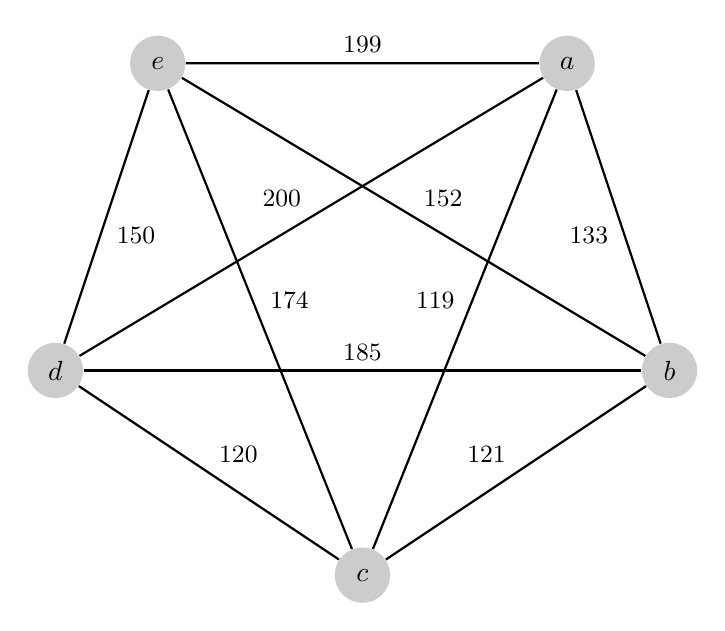
\begin{tikzpicture}[scale=1.3, auto,swap]

% Draw a network

% First we draw the vertices
\foreach \pos/\name in {{(2,2)/a}, {(3,-1)/b}, {(0,-3)/c}, {(-3,-1)/d}, {(-2,2)/e}}
\node[vertex] (\name) at \pos {$\name$};

% Connect vertices with edges and draw weights
\foreach \source / \dest / \weight in {a/b/133, a/c/119, a/d/200, a/e/199, b/c/121, b/d/185, b/e/152, c/d/120, c/e/174, d/e/150}
\path[edge] (\source) -- node[weight] {$\weight$} (\dest);

\end{tikzpicture}
\end{figure}

\end{frame}

%-----------------------------------%

\begin{frame}
\frametitle{Nearest Neighbor Algorithm \\ (Starting at Vertex $d$)}


%% Adjacency matrix of graph
%% \   a   b   c   d   e  
%% a   x  133 119 200 199 
%% b   -   x  121 185 152
%% c   -   -   x  120 174
%% d   -   -   -   x  150
%% e   -   -   -   -   x

\begin{figure}
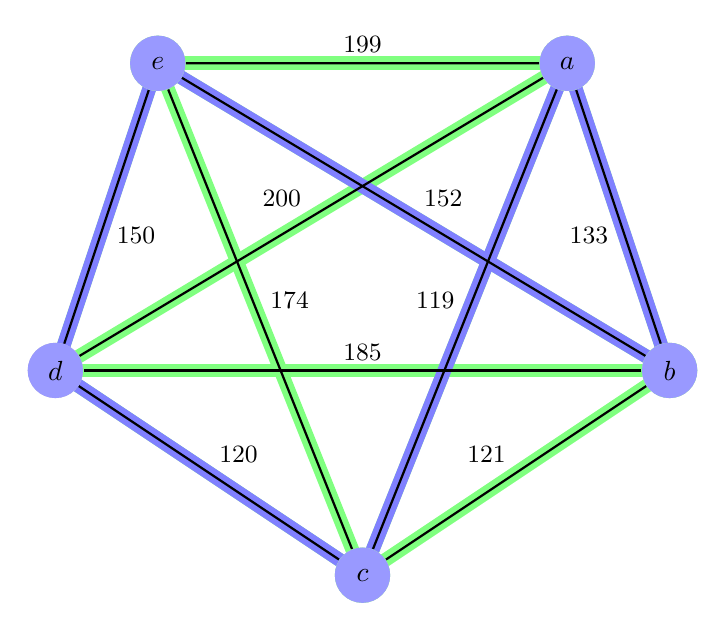
\begin{tikzpicture}[scale=1.3, auto,swap]

% Draw a network

% First we draw the vertices
\foreach \pos/\name in {{(2,2)/a}, {(3,-1)/b}, {(0,-3)/c}, {(-3,-1)/d}, {(-2,2)/e}}
\node[vertex] (\name) at \pos {$\name$};

% Connect vertices with edges and draw weights
\foreach \source / \dest / \weight in {a/b/133, a/c/119, a/d/200, a/e/199, b/c/121, b/d/185, b/e/152, c/d/120, c/e/174, d/e/150}
\path[edge] (\source) -- node[weight] {$\weight$} (\dest);

%%%%%%%%%%%%%%%%%%%%%%%%%%%%%%%%%%%%%%%%%%%%%%%%%%        
% Start animating the vertex and edge selection. % 
%%%%%%%%%%%%%%%%%%%%%%%%%%%%%%%%%%%%%%%%%%%%%%%%%%
% Possible vertex animation
\foreach \vertex / \fr in {a/1,b/1,c/1,e/1}
\path<\fr-> node[possible vertex] at (\vertex) {$\vertex$};        

% Selected vertex animation
\foreach \vertex / \fr in {d/1,c/3,a/5,b/7,e/9}
  \path<\fr-> node[selected vertex] at (\vertex) {$\vertex$};

%%%%%%%%%%%%%%%%%%
% Edge animation %
%%%%%%%%%%%%%%%%%%
\begin{pgfonlayer}{background}

% Possible edge animation
\foreach \source / \dest / \startfr / \endfr in {d/a/2/3,d/b/2/3,d/e/2/3,d/c/2/3,
c/a/4/5,c/b/4/5,c/e/4/5,
a/b/6/7,a/e/6/7,
b/e/8/9}
\path<\startfr-\endfr>[possible edge] (\source.center) --  (\dest.center);

% Selected edge animation
\foreach \source / \dest / \fr in {d/c/3,c/a/5,a/b/7,b/e/9,e/d/10}
\path<\fr->[selected edge] (\source.center) --  (\dest.center);

\end{pgfonlayer}

\end{tikzpicture}
\end{figure}


\end{frame}

%-----------------------------------%

\begin{frame}
\frametitle{Sorted Edges (Cheapest Link) Algorithm}

%% Adjacency matrix of graph
%% \   a   b   c   d   e  
%% a   x  133 119 200 199 
%% b   -   x  121 185 152
%% c   -   -   x  120 174
%% d   -   -   -   x  150
%% e   -   -   -   -   x

\begin{figure}
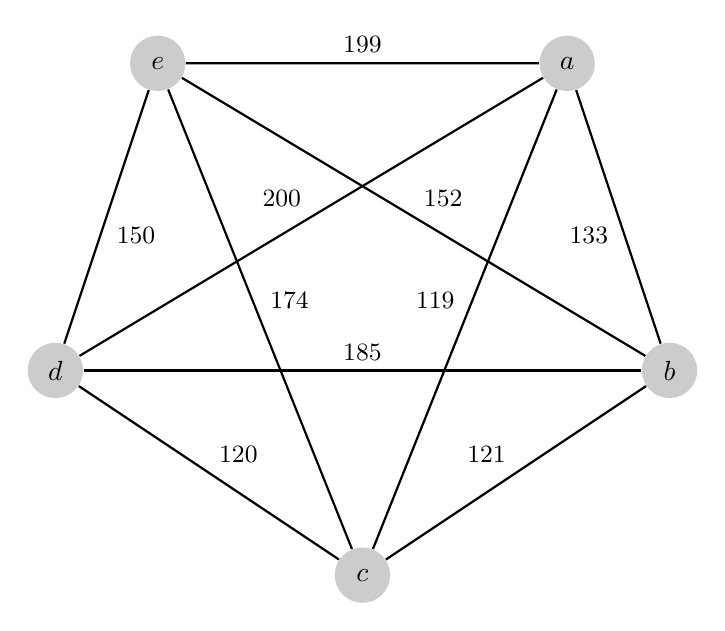
\begin{tikzpicture}[scale=1.3, auto,swap]

% Draw a network
    
% First we draw the vertices
\foreach \pos/\name in {{(2,2)/a}, {(3,-1)/b}, {(0,-3)/c},{(-3,-1)/d}, {(-2,2)/e}}
\node[vertex] (\name) at \pos {$\name$};
        
% Connect vertices with edges and draw weights
\foreach \source/ \dest /\weight in {a/b/133, a/c/119, a/d/200, a/e/199, b/c/121, b/d/185, b/e/152, c/d/120, c/e/174, d/e/150}
\path[edge] (\source) -- node[weight] {$\weight$} (\dest);
\end{tikzpicture}
\end{figure}
\end{frame}

%~~~~~~~~~~~~~%

\begin{frame}
\frametitle{Sorted Edges (Cheapest Link) Algorithm}

The weights of the edges are:

$$
133,\ 119,\ 200,\ 199,\ 121,\ 185,\ 152,\ 120,\ 174,\ 150.
$$
\pause
First, we need to sort the edge-weights:
\pause
$$
119,\ 120,\ 121,\ 133,\ 150,\ 152,\  174,\ 185,\ 199,\ 200.
$$
\pause
Now we can proceed to construct a Hamiltonian circuit using the Cheapest Link Algorithm.
\end{frame}

%~~~~~~~~~~~~~%

\begin{frame}
\frametitle{Sorted Edges (Cheapest Link) Algorithm}

%%%%%%%%%%%%%%%
\begin{center}
$
\hilight<2->{119},\, \hilight<2->{120},\, \xcancel<4->{121},\, \hilight<6->{133},\, \hilight<7->{150},\, \hilight<8->{152},\,  \xcancel<9->{174,\, 185,\, 199,\, 200}.
$
\end{center}
%%%%%%%%%%%%%%%

%% Adjacency matrix of graph
%% \   a   b   c   d   e  
%% a   x  133 119 200 199 
%% b   -   x  121 185 152
%% c   -   -   x  120 174
%% d   -   -   -   x  150
%% e   -   -   -   -   x

\begin{figure}
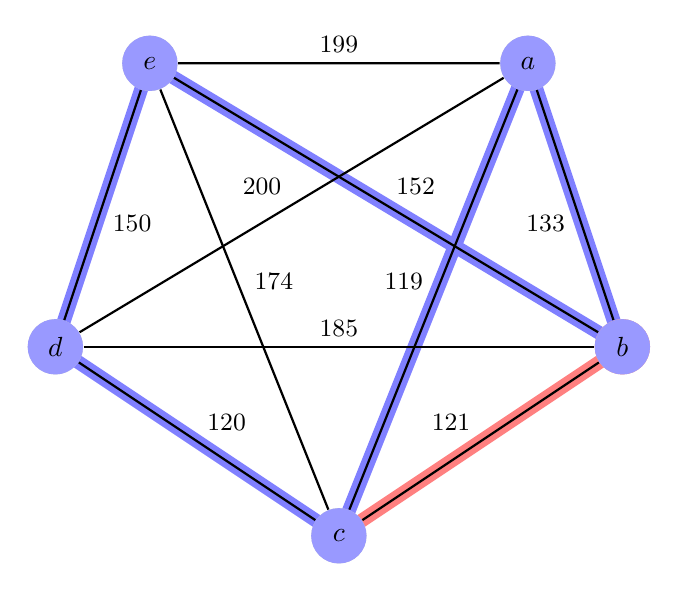
\begin{tikzpicture}[scale=1.2, auto,swap]

% Draw a network

% First we draw the vertices
\foreach \pos/\name in {{(2,2)/a}, {(3,-1)/b}, {(0,-3)/c}, {(-3,-1)/d}, {(-2,2)/e}}
\node[vertex] (\name) at \pos {$\name$};

% Connect vertices with edges and draw weights
\foreach \source/ \dest /\weight in {a/b/133, a/c/119, a/d/200, a/e/199, b/c/121, b/d/185, b/e/152, c/d/120, c/e/174, d/e/150}
\path[edge] (\source) -- node[weight] {$\weight$} (\dest);

%%%%%%%%%%%%%%%%%%%%%%%%%%%%%%%%%%%%%%%%%%%%%%%%%%        
% Start animating the vertex and edge selection. % 
%%%%%%%%%%%%%%%%%%%%%%%%%%%%%%%%%%%%%%%%%%%%%%%%%%
% Bad vertex animation
\foreach \vertex / \startfr / \endfr in {b/3/4}
  \path<\startfr-\endfr> node[bad vertex] at (\vertex) {$\vertex$};     

% Selected vertex animation
\foreach \vertex / \fr in {d/2,c/2,a/2,b/6,e/7}
  \path<\fr-> node[selected vertex] at (\vertex) {$\vertex$};
  
%%%%%%%%%%%%%%%%%%
% Edge animation %
%%%%%%%%%%%%%%%%%%
\begin{pgfonlayer}{background}

% Bad edge animation
\foreach \source / \dest / \startfr / \endfr in {b/c/3/4}
\path<\startfr-\endfr>[bad edge] (\source.center) --  (\dest.center);

% Selected edge animation
\foreach \source / \dest / \fr in {a/c/2,c/d/2,a/b/6,d/e/7,b/e/8}
\path<\fr->[selected edge] (\source.center) --  (\dest.center);

\end{pgfonlayer}

\end{tikzpicture}
\end{figure}

\end{frame}

%-----------------------------------%

\subsection{Kruskal's Algorithm}

\begin{frame}
\frametitle{Kruskal's Algorithm}

\begin{figure}
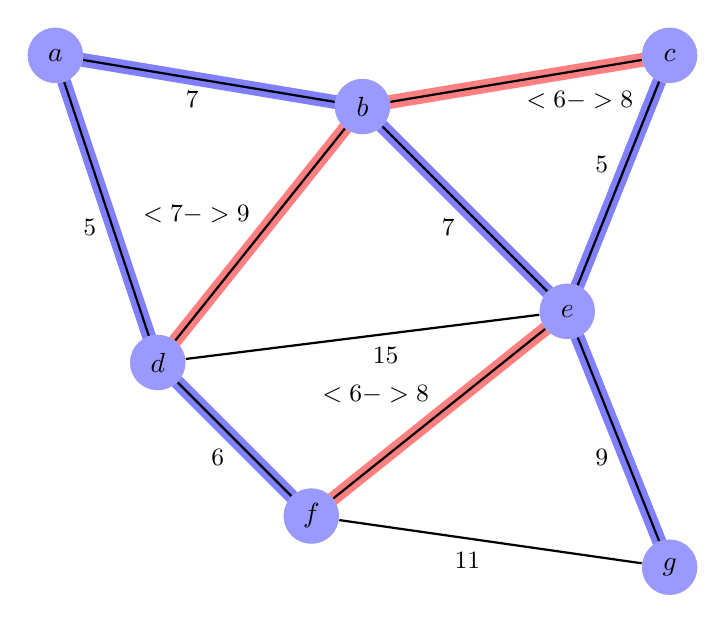
\begin{tikzpicture}[scale=1.3, auto,swap]

%% Adjacency matrix of graph
%% \   a   b   c   d   e   f   g   
%% a   x   7   i   5   i   i   i
%% b   -   x   8   9   7   i   i
%% c   -   -   x   i   5   i   i
%% d   -   -   -   x   15  6   i
%% e   -   -   -   -   x   8   9
%% f   -   -   -   -   -   x   11
%% g   -   -   -   -   -   -   x

% Draw a network

% First we draw the vertices
\foreach \pos / \name in {{(-3,4)/a},{(0,3.5)/b},{(3,4)/c},{(-2,1)/d},{(2,1.5)/e},{(-0.5,-0.5)/f},{(3,-1)/g}}
\node[vertex] (\name) at \pos {$\name$};

% Connect vertices with edges and draw weights
\foreach \source/ \dest / \weight in {a/b/7,a/d/5,b/c/\xcancel<6->{8},b/d/\xcancel<7->{9},b/e/7,c/e/5,d/e/15,d/f/6,e/f/\xcancel<6->{8},e/g/9,f/g/11}
\path[edge] (\source) -- node[weight] {$\weight$} (\dest);

%%%%%%%%%%%%%%%%%%%%%%%%%%%%%%%%%%%%%%%%%%%%%%%%%%        
% Start animating the vertex and edge selection. % 
%%%%%%%%%%%%%%%%%%%%%%%%%%%%%%%%%%%%%%%%%%%%%%%%%%  
% Bad vertex animation
\foreach \vertex / \startfr / \endfr in {}
  \path<\startfr-\endfr> node[bad vertex] at (\vertex) {$\vertex$};     

% Selected vertex animation
\foreach \vertex / \fr in {a/2,c/2,d/2,e/2,f/3,b/4,g/6}
  \path<\fr-> node[selected vertex] at (\vertex) {$\vertex$};
  
%%%%%%%%%%%%%%%%%%
% Edge animation %
%%%%%%%%%%%%%%%%%%
\begin{pgfonlayer}{background}

% Bad edge animation
\foreach \source / \dest / \startfr / \endfr in {b/c/5/5,e/f/5/5,b/d/6/6}
\path<\startfr-\endfr>[bad edge] (\source.center) --  (\dest.center);

% Selected edge animation
\foreach \source / \dest / \fr in {a/d/2,c/e/2,d/f/3,a/b/4,b/e/4,e/g/6,e/g/7}
\path<\fr->[selected edge] (\source.center) --  (\dest.center);

\end{pgfonlayer}

\end{tikzpicture}
\end{figure}

\end{frame}


%-----------------------------------%

\subsection{Eulerian Circuits}

\begin{frame}
\frametitle{Eulerization}
\begin{figure}
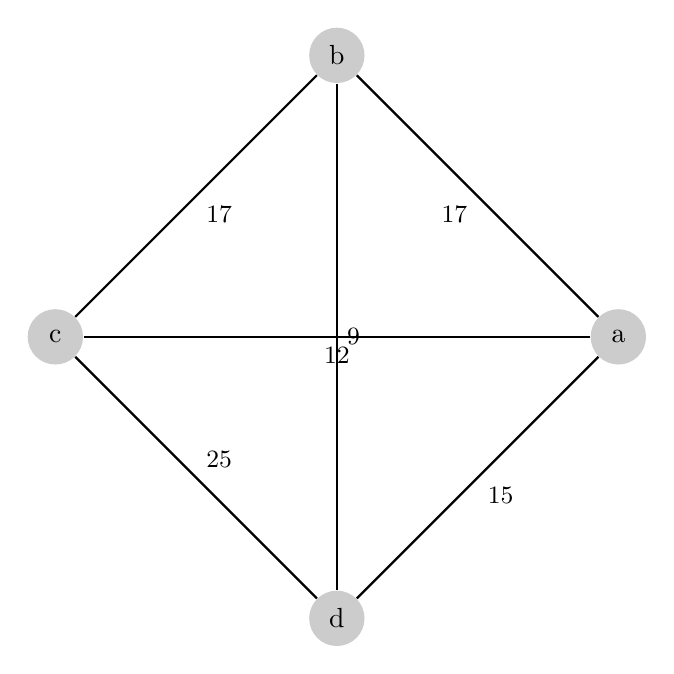
\begin{tikzpicture}[auto,scale=1.1]
\net{4}{a,b,c,d}{%
{x,\rn,\rn,\rn},
{-,x,\rn,\rn},
{-,-,x,\rn},
{-,-,-,x}
}%
\end{tikzpicture}
\end{figure}
\end{frame}

%-----------------------------------%

\begin{frame}
\frametitle{Eulerization}

\begin{figure}
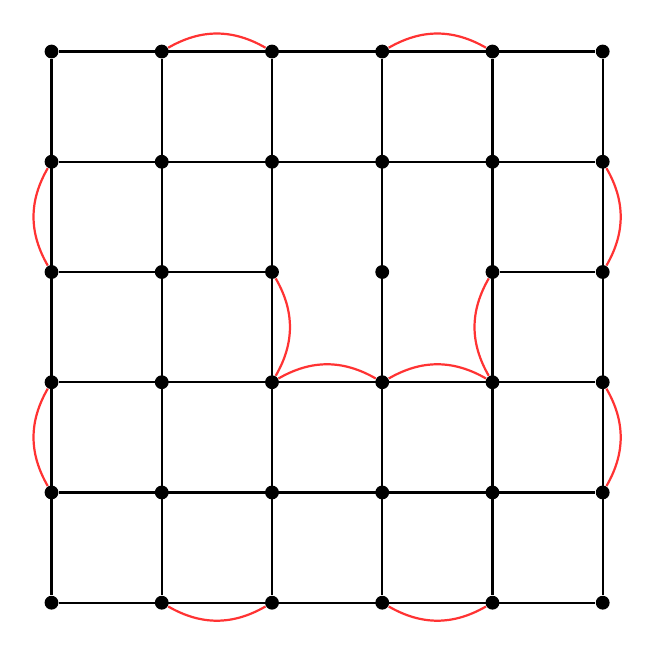
\begin{tikzpicture}[scale=1.4, auto,swap]

% Draw a network

% First we draw the vertices
\foreach \pos / \name in {{(-2.5,2.5)/1},
{(-1.5,2.5)/2},
{(-0.5,2.5)/3},
{(0.5,2.5)/4},
{(1.5,2.5)/5},
{(2.5,2.5)/6},
{(-2.5,1.5)/7},
{(-1.5,1.5)/8},
{(-0.5,1.5)/9},
{(0.5,1.5)/10},
{(1.5,1.5)/11},
{(2.5,1.5)/12},
{(-2.5,0.5)/13},
{(-1.5,0.5)/14},
{(-0.5,0.5)/15},
{(0.5,0.5)/16},
{(1.5,0.5)/17},
{(2.5,0.5)/18},
{(-2.5,-0.5)/19},
{(-1.5,-0.5)/20},
{(-0.5,-0.5)/21},
{(0.5,-0.5)/22},
{(1.5,-0.5)/23},
{(2.5,-0.5)/24},
{(-2.5,-1.5)/25},
{(-1.5,-1.5)/26},
{(-0.5,-1.5)/27},
{(0.5,-1.5)/28},
{(1.5,-1.5)/29},
{(2.5,-1.5)/30},
{(-2.5,-2.5)/31},
{(-1.5,-2.5)/32},
{(-0.5,-2.5)/33},
{(0.5,-2.5)/34},
{(1.5,-2.5)/35},
{(2.5,-2.5)/36}}
\node[Euler vertex] (\name) at \pos {$ $};

% Connect vertices with edges and draw weights
\foreach \source/ \dest in {1/6,7/12,13/15,17/18,19/24,25/30,31/36,1/31,2/32,3/33,4/34,5/35,6/36}
\path[edge] (\source) -- (\dest);

\tikzstyle{EdgeStyle}=[color=red!80,bend left]
\Edge(2)(3)
\Edge(4)(5)
\Edge(12)(18)
\Edge(24)(30)
\Edge(15)(21)
\Edge(21)(22)
\Edge(22)(23)
\Edge(23)(17)

\tikzstyle{EdgeStyle}=[color=red!80,bend right]
\Edge(7)(13)
\Edge(19)(25)
\Edge(32)(33)
\Edge(34)(35)

\end{tikzpicture}
\end{figure}

\end{frame}


%-----------------------------------%

\subsection{Hamiltonian Graphs}

\begin{frame}
\frametitle{Hamiltonian Circuits}

\begin{figure}
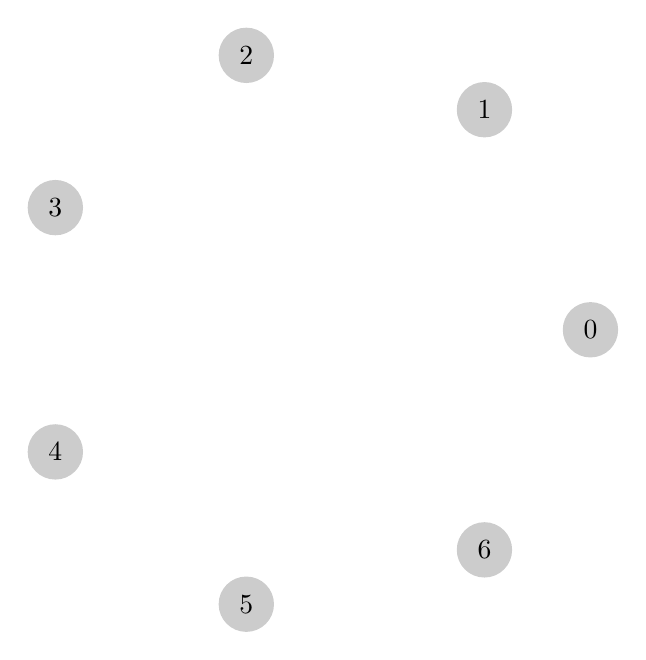
\begin{tikzpicture}[auto,scale=1.1]
\net{7}{}{}
\end{tikzpicture}
\end{figure}

\end{frame}

%-----------------------------------%

\begin{frame}
\frametitle{Experiment}

\def\myset{a,b,c,d,e}

\def\myex{c}

\myset

\myex

\foreach \myel in \myset
{%
  \if\myex\myel
  {%
  }%
  \else
  {%
    \myel
  }%
  \fi
}%

\end{frame}

%-----------------------------------%

\begin{frame}
\frametitle{Experiment}

\begin{figure}
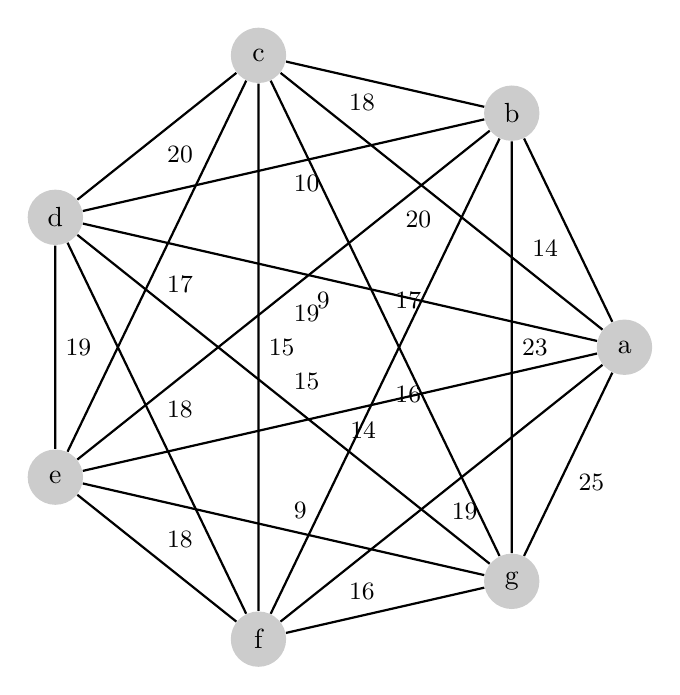
\begin{tikzpicture}[auto,scale=1.17]
\net{7}{a,b,c,d,e,f,g}{%
{x,\rn,\rn,\rn,\rn,\rn,\rn}, % 1
{-,x,\rn,\rn,\rn,\rn,\rn},   % 2
{-,-,x,\rn,\rn,\rn,\rn},     % 3
{-,-,-,x,\rn,\rn,\rn},       % 4
{-,-,-,-,x,\rn,\rn},         % 5
{-,-,-,-,-,x,\rn},           % 6
{-,-,-,-,-,-,x},             % 7
}%
\end{tikzpicture}
\end{figure}

\end{frame}

%-----------------------------------%


% 101 TAs - E-mail List:
%
% --REMOVED--
%
\end{document}
